% !TEX encoding = UTF-8
% !TEX TS-program = pdflatex
% !TEX root = ../tesi.tex
% !TEX spellcheck = it-IT

%**************************************************************
\chapter{Progettazione e sviluppo}
\label{cap:progettazione-codifica}
%**************************************************************

\intro{In questo capitolo vengono presentate le tecnologie e gli strumenti adottati e vengono spiegate le scelte progettuali adottate}\\

%**************************************************************
\section{Tecnologie e strumenti}
\label{sec:tecnologie-strumenti}

L'azienda ha lasciato grande libertà riguardo agli strumenti e le tecnologie da utilizzare per questo progetto, quindi essi sono stati fissati inizialmente e successivamente incrementati al crescere delle necessità.

\subsection{Codice}
Segue la lista dei linguaggi utilizzati per la codifica.
\begin{itemize}
	\item \textbf{Java\footnote{https://www.java.com}}: Il linguaggio preferito per l'applicazione lato \emph{tablet}. È stato scelto seguendo le \emph{Best Practice} dello sviluppo \emph{Android}.
	\item \textbf{C++\footnote{www.cplusplus.com}}: Il linguaggio preferito per l'applicazione lato \emph{Server}. È stato scelto perché tutte le più diffuse librerie per l'elaborazione dei \emph{Point Cloud}, ed in particolare \emph{PCL} sono disponibili in questo linguaggio.
	\item \textbf{PHP\footnote{https://secure.php.net}}: Il linguaggio usato per ricevere ed inviare le richieste \emph{HTTP} necessarie alla comunicazione tra \emph{Server} e dispositivo.
	\item \textbf{Python\footnote{https://www.python.org}}: Il linguaggio usato in combinazione con \emph{PHP} per elaborare le richieste ed implementare la logica del lato \emph{Server}. Essendo un linguaggio particolarmente adatto alla computazione numerica è stato usato inoltre per il calcolo del volume di una mesh.
\end{itemize}

\newpage
\subsection{IDE ed editor}
Segue la lista degli ambienti per la codifica utilizzati durante il progetto.
\begin{itemize}
	\item \textbf{Android Studio\footnote{https://developer.android.com/studio/index.html}}: L'\emph{IDE} ufficiale per le applicazioni \emph{Android}.
	\item \textbf{QT\footnote{https://www.qt.io/ide}}: L'\emph{IDE} scelto per lo sviluppo del codice \emph{C++}.
	\item \textbf{Geany\footnote{https://www.geany.org}}: L'\emph{editor} di testo usato per scrivere gli \emph{script} \emph{PHP} e \emph{Python}.
\end{itemize}

\subsection{Framework}
Segue la lista dei \emph{Framework} usati per il tirocinio.
\begin{itemize}
	\item \textbf{PCL, Point Cloud Library\footnote{http://pointclouds.org}}: Una  delle librerie di maggior rilievo nel campo della \emph{Computer Vision}, \emph{Open Source}, scritta in C++, di algoritmi per l'elaborazione di \emph{Point Cloud} tridimensionali. Contiene algoritmi per il filtraggio, la segmentazione, la \emph{registration} e il \emph{meshing} di Point Cloud, per citarne alcuni. \\
La libreria è ampiamente utilizzata da qualsiasi applicativo debba trattare nuvole di punti, ed oltre ad essere utile ed efficiente è anche ben documentata, con molti esempi d'utilizzo reperibili online.\\
Le notevoli potenzialità della libreria sono state utilizzate intensivamente nell'applicativo con lo scopo di isolare i punti appartenenti all'oggetto scansionato dal resto del Point Cloud, ed effettuarne quindi il meshing.

	\item \textbf{Tango API\footnote{https://developers.google.com/tango/apis/overview}}: Le \emph{API} ufficiali, disponibili in linguaggio Java, C++ e C\#, per lo sviluppo di applicazioni \emph{Tango}.
	\item \textbf{Gradle\footnote{https://gradle.org}}: È stato usato come \emph{tool} di \emph{build} per tutta l'applicazione \emph{Android}. \'E inoltre il \emph{build-tool} di default dell'ambiente \emph{Android Studio}.
	\item \textbf{OkHttp\footnote{http://square.github.io/okhttp}}: È stata usato come \emph{framework} di riferimento per le richieste \emph{http}, come indicato nella \emph{Android Best Practices}.
	\item \textbf{TangoUx\footnote{https://developers.google.com/tango/ux/ux-framework}}: \emph{Famework} messo a disposizione da \emph{Google} assieme alle \emph{API Tango}. È stato usato per gestire le notifiche all'utente relative ai comportamenti che deve tenere per permettere il buon funzionamento del dispositivo e dei sensori.
	\item \textbf{Jni\footnote{http://docs.oracle.com/javase/7/docs/technotes/guides/jni}}: Questo \emph{framework} permette di richiamare metodi 'nativi' (scritti in \emph{C/C++}) dal codice \emph{Java}. \'E stato usato nell'ultimo prototipo dell'applicazione, per esplorare le funzionalità della libreria (scritta in C++) GOICP.
	\item \textbf{Firebase\footnote{https://firebase.google.com}}: \emph{Framework} associato all'omonimo \emph{web service} offerto da \emph{Google} per lo scambio di messaggi tra applicazioni \emph{Android} e un \emph{server}.
	\item \textbf{GOICP\footnote{http://iitlab.bit.edu.cn/mcislab/~yangjiaolong/go-icp/}}: libreria che implementa una variante dell'algoritmo ICP per la \emph{Registration} di set di \emph{Point Cloud}.
\end{itemize}

\subsection{Server}
L'applicativo lato server è stato sviluppato e testato su un web server \emph{Apache}\footcite{https://httpd.apache.org/}, preferito per la sua facilità di configurazione, modularità ed affidabilità. Il server \emph{Apache} è stato installato sulla macchina del tirocinante.

\newpage
%**************************************************************
\section{Progettazione}
\label{sec:progettazione}
Sulla base dei requisiti analizzati nel capitolo \emph{Analisi dei requisiti}(cap. \ref{cap:analisi-requisiti}) si è svolta la progettazione dell'applicativo. Prima di tutto si è reso necessario suddividere la progettazione lato client dal lato server; quanto svolto nell'applicativo lato client andava infatti inserito ed integrato in un prototipo già esistente, mentre il lato server doveva essere progettato da zero.
Vediamo ora le scelte progettuali adottate.

\subsection{Architettura lato client}
Al lato client è stato necessario prendere coscienza dell'architettura e della logica dell'applicazione prototipale già realizzata, per poter sviluppare un nuovo prototipo che inserisca nuove funzionalità integrandole correttamente nel sistema. 
Il prototipo sviluppato, denominato \emph{VIC-Tango}, partendo dallo stadio prototipale precedente dell'applicazione (\emph{Samba}), introduce le seguenti migliorie e funzionalità:
\begin{itemize}
\item Possibilità di caricare in una lista le \emph{mesh} risultato dell'elaborazione lato server di un \emph{Point Cloud}, e poter visualizzare il singolo render di una mesh.
\item Un servizio di notifica che riceve messaggi sull'esito dell'elaborazione di un \emph{Point Cloud} da parte del server.
\item Miglioramento della Camera Preview dell'applicazione.
\item Introdotti i framework JNI e GOICP per testare funzionalità di Point Cloud Registration.
\end{itemize}
Vediamo le scelte progettuali adottate per implementare tali funzionalità.

\subsubsection{Lista di mesh}
Per implementare una lista di mesh e la possibilità di visualizzare il render di una singola mesh, tutte le classi e le funzionalità associate sono state inserite in un nuovo package \texttt{rendering}, come da figura \ref{fig:meshList}.
\begin{figure}[!h] 
    \centering 
    \includegraphics[width=1.0\columnwidth]{client/meshList.png} 
    \caption{Diagramma UML del package \texttt{rendering}}
   \label{fig:meshList}
\end{figure}
Il package contiene le seguenti classi:
\begin{itemize}
\item \texttt{MeshListActivity}: L'activity principale della funzionalità di visualizzazione della lista di mesh.
\item \texttt{MeshListManager}: Manager responsabile di gestire la business logic di MeshListActivity, separando così la presentazine dalla logica.
\end{itemize}
Ed i seguenti sub-package:
\begin{itemize}
\item\texttt{receivers}: Contiene le classi necessarie a ricevere dati dal server, sotto forma di oggetti JSON. Il package, come da figura \ref{fig:receivers}, contiene le seguenti classi:
\begin{figure}[!h] 
    \centering 
    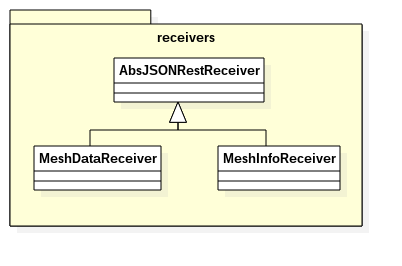
\includegraphics[width=0.7\columnwidth]{client/receivers.png} 
    \caption{Diagramma UML del package \texttt{receivers}}
   \label{fig:receivers}
\end{figure}
\begin{itemize}
	\item\texttt{AbsJSONRestReceiver}: Classe astratta che rappresenta un interfaccia REST per la richiesta e ricezione di dati in formato JSON.
	\item\texttt{MeshDataReceiver}: Implementazione di \texttt{AbsJSONRestReceiver} che richiede e riceve file OBJ dal server come oggetti JSON.
	\item\texttt{MeshInfoReceiver}: Implementazione di \texttt{AbsJSONRestReceiver} che richiede e riceve informazioni sulle mesh salvate sul server come array di oggetti JSON.
	\end{itemize}
\item\texttt{tasks}: Contiene classi che eseguono asincronamente compiti temporalmente dispendiosi, quali il caricamento e salvataggio delle mesh e il caricamento da server. Il package, come da figura \ref{fig:tasks}, contiene le seguenti classi:
\begin{figure}[!h] 
    \centering 
    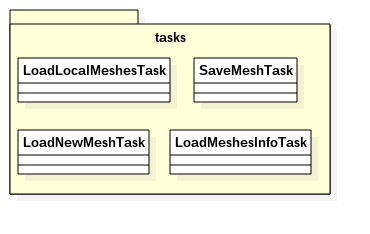
\includegraphics[width=0.6\columnwidth]{client/tasks.png} 
    \caption{Diagramma UML del package \texttt{tasks}}
   \label{fig:tasks}
\end{figure}
	\begin{itemize}
	\item\texttt{LoadLocaMeshesTask}: Classe per il caricamento asincrono delle mesh salvate localmente sul \emph{device}.
	\item\texttt{LoadMeshesInfoTask}: Classe per il caricamento asincrono delle informazioni sulle mesh salvate nel server. 
	\item\texttt{LoadNewMeshTask}: Classe per il caricamento asincrono di una mesh dal server.
	\item\texttt{SaveMeshTask}: Classe per il salvataggio asincrono di una mesh ricevuta sulla memoria locale del \emph{device}. La mesh viene salvata in un file OBJ.
	\end{itemize}
\item\texttt{services}: Contiene classi che implementano servizi che necessitano di essere per lungo tempo in background. Il package, come da figura \ref{fig:services}, contiene le seguenti classi:
\begin{figure}[!h] 
    \centering 
    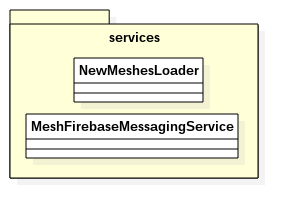
\includegraphics[width=0.5\columnwidth]{client/services.png} 
    \caption{Diagramma UML del package \texttt{services}}
   \label{fig:services}
\end{figure}
	\begin{itemize}
	\item\texttt{NewMeshesLoader}: Servizio che effettua il refresh della lista di mesh locali caricando dal server le nuove mesh disponibili.
	\item\texttt{MeshFirebaseMessagingService}: Servizio che, in background, aspetta di ricevere messaggi dal server attraverso il web-service Firebase, ed alla ricezione di un messaggio genera una notifica di sistema \emph{Android} per informare l'utente.
	\end{itemize}
\item\texttt{model3D}: Contiene classi per il rendering e la visualizzazione di mesh (file OBJ). Il package corrisponde all'applicazione open source \emph{3D Model Viewer Open Source\footcite{https://play.google.com/store/apps/details?id=org.andresoviedo.dddmodel&hl=it}} che in quanto non implementata dal tirocinante, non verrà qui documentata.
\end{itemize}

\subsubsection{Camera Preview}
La \emph{Camera Preview}, cioè un piccolo riquardo nell'applicazione che mostra quanto ripreso dalla fotocamera, è stata reimplementata, abbandonando la vecchia implementazione \texttt{VideoRenderer}, che soffriva di problemi di stabilità e prestazioni. \'E stata creata quindi nel package \texttt{camera} (vedi fig. \ref{fig:camera}) una classe \texttt{RGBBoxManager} che sfrutta funzionalità delle \emph{Tango API} per il controllo della fotocamera RGB-IR dei \emph{device Tango}, ottenendo così una preview più affidabile e fluida.
\begin{figure}[!h] 
    \centering 
    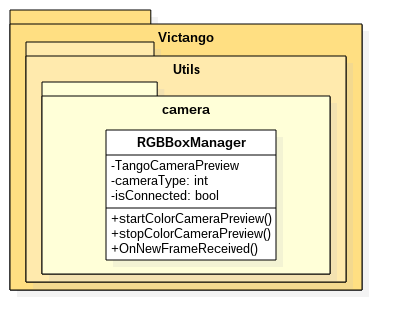
\includegraphics[width=0.7\columnwidth]{client/camera.png} 
    \caption{Diagramma UML del package \texttt{camera}}
   \label{fig:camera}
\end{figure}

\subsubsection{JNI e Point Cloud Registration}
In \emph{VIC-Tango} è stata aggiunta una nuova strategia di ricostruzione del Point Cloud, rispettando l'architettura già presente e sfruttando il pattern \emph{strategy}, una nuova classe \texttt{GOICPPCloudReconstruction} nel package \texttt{Reconstruction}, che sfrutta le funzionalità della libreria esterna GOICP, come da figura \ref{fig:GOICPRec}.
\begin{figure}[!h] 
    \centering 
    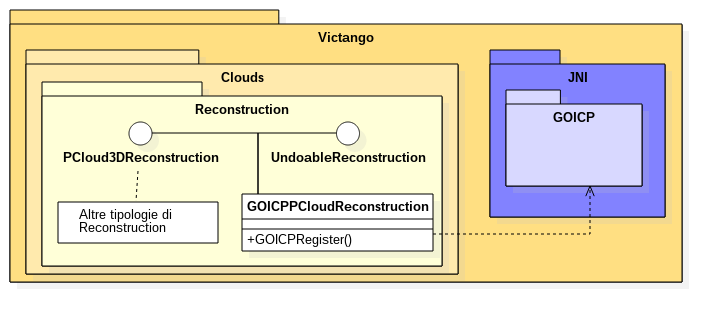
\includegraphics[width=1.0\columnwidth]{client/GOICPRec.png} 
    \caption{Diagramma UML del package \texttt{Reconstruction}}
   \label{fig:GOICPRec}
\end{figure}
Inoltre per integrare la libreria GOICP, scritta nativamente in C++, è stato necessario importare nel progetto il framework JNI, che permette di richiamare codice nativo da codice Java.
\newpage



\subsection{Architettura lato server}
Il lato server dell'applicazione è stato progettato da zero, basandosi quindi sui requisiti rilevati in fase d'analisi e sulle necessità del committente.
L'architettura server espone una serie di servizi al client, quali la ricezione di file PCD, o l'invio di mesh ed info sulle mesh salvate, oltre ovviamente all'elaborazione dei \emph{Point Cloud ricevuti}.
\begin{figure}[!h] 
    \centering 
    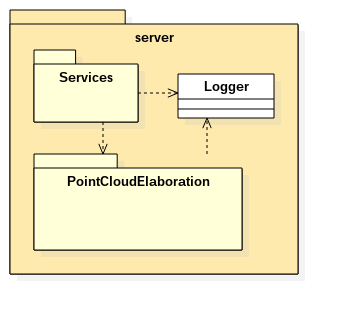
\includegraphics[width=0.6\columnwidth]{server/server.png} 
    \caption{Diagramma UML del package \texttt{server}}
   \label{fig:server}
\end{figure}
Come evidenziato in figura \ref{fig:server} il lato server è così suddiviso:
\begin{itemize}
\item\texttt{Services}: Package che espone le funzionalità del server al client.
\item\texttt{PointCloudElaboration}: Package che contiene tutte le funzionalità necessarie all'elaborazione di un \emph{Point Cloud}.
\item\texttt{Logging}: Singleton che espone funzionalità di logging per i servizi del server e per il processo di elaborazione dei \emph{Point Cloud}.
\end{itemize}
Vediamo in maggior dettaglio le componenti dell'architettura.

\subsubsection{Services}
Il package services racchiude le funzionalità del server, rappresentate in figura \ref{fig:Services} dalle seguenti classi:
\begin{figure}[!h] 
    \centering 
    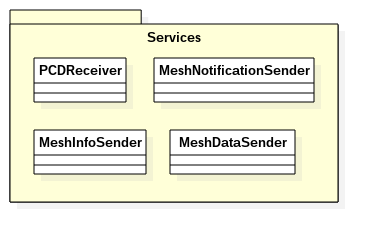
\includegraphics[width=0.6\columnwidth]{server/Services.png} 
    \caption{Diagramma UML del package \texttt{Services}}
   \label{fig:Services}
\end{figure}
\begin{itemize}
\item\texttt{PCDReceiver}: Classe responsabile di ricevere dal client i \emph{Point Cloud} acquisiti e di salvarli su un file PCD locale. Una volta salvato il \emph{Point Cloud} su file PCD ne viene avviata l'elaborazione.
\item\texttt{MeshDataSender}: Classe responsabile di inviare una specifica mesh via protocollo HTTP al Client.
\item\texttt{MeshInfoSender}: Classe responsabile di inviare una serie di informazioni quali nome, data di creazione e volume delle mesh salvate, via protocollo HTTP, al client.
\item\texttt{MeshNotificationSender}: Classe responsabile di inviare un messaggio riguardante l'esito dell'elaborazione di un Point Cloud al web-service Firebase. Firebase provvederà poi autonomamente a recapitare il messaggio al \emph{device Tango}.
\end{itemize}

\subsubsection{PointCloudElaboration}
Il package racchiude tutte le funzionalità di manipolazione, filtraggio, meshing e calcolo del volume di un Point Cloud. 
Come da figura\ref{fig:PCElaboration} il package è formato dalle seguenti classi:
\begin{figure}[!h] 
    \centering 
    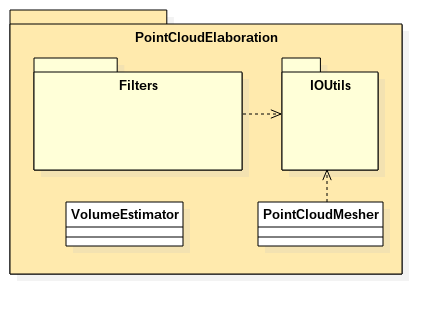
\includegraphics[width=0.6\columnwidth]{server/PCElaboration.png} 
    \caption{Diagramma UML del package \texttt{PointCloudElaboration}}
   \label{fig:PCElaboration}
\end{figure}
\begin{itemize}
\item\texttt{VolumeEstimator}: Classe che espone le funzionalità per il calcolo del volume di una mesh. Il volume viene calcolato leggendo il file VTK prodotto da \texttt{PointCloudMesher} dopo l'elaborazione di un Point Cloud.
\item\texttt{PointCloudMesher}: Classe che espone le funzionalità per il meshing di un PointCloud, può salvare la mesh prodotta in formato OBJ e VTK.
\end{itemize}
E dai seguenti sub-package:
\begin{itemize}
\item\texttt{Filters}:
	Il package racchude tutte le funzionalità per il filtraggio e l'eliminazione di punti da un Point Cloud. \'E formato dalle seguenti classi:
	\begin{figure}[!h] 
	    \centering 
	    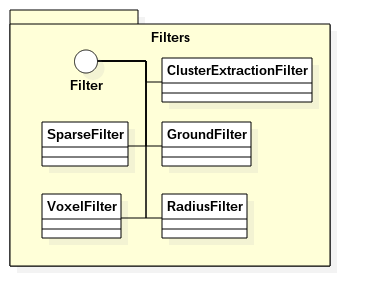
\includegraphics[width=0.6\columnwidth]{server/Filters.png} 
	    \caption{Diagramma UML del package \texttt{Filters}}
	   \label{fig:Filters}
	\end{figure}
	\begin{itemize}
	\item\texttt{Filter}: Interfaccia che definisce le operazioni di base per il filtraggio di Point CLoud
	\item\texttt{SparseFilter}: Classe che implementa \texttt{Filter} per il filtraggio dei punti isolati di un Point Cloud.
	\item\texttt{RadiusFilter}: Classe che implementa \texttt{Filter} per il filtraggio dei punti esterni (non appartenenti all'oggetto scansionato) di un Point Cloud.
	\item\texttt{VoxelFilter}: Classe che implementa \texttt{Filter} per il filtraggio dei punti doppi o eccessivamente ravvicinati di un Point Cloud.
	\item\texttt{GroundFilter}: Classe che implementa \texttt{Filter} per il filtraggio dei punti che rappresentano il piano del pavimento di un Point Cloud.
	\item\texttt{ClusterExtractionFilter}: Classe che implementa \texttt{Filter} per l'estrazione da un Point Cloud della sola nuvola di punti rappresentante l'oggetto scansionato.
	\end{itemize}

\item\texttt{IOUtils}:
	Il package racchiude tutte le funzionalità per il salvataggio e caricamento di file inerenti all'applicativo, quindi i formati PCD, OBJ e VTK. \'E formato dalle classi:
	\begin{figure}[!h] 
	    \centering 
	    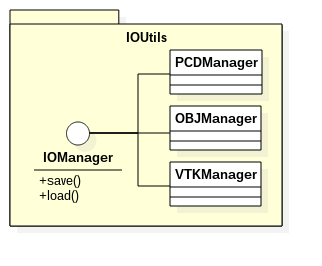
\includegraphics[width=0.55\columnwidth]{server/IOUtils.png} 
	    \caption{Diagramma UML del package \texttt{IOUtils}}
	   \label{fig:IOUtils}
	\end{figure}
	\begin{itemize}
	\item\texttt{IOManager}: Interfaccia che definisce le operazioni di base per un manager di Input/Output.
	\item\texttt{PCDManager}: Classe che implementa \texttt{IOManager} per il salvataggio e caricamento di file PCD.
	\item\texttt{OBJManager}: Classe che implementa \texttt{IOManager} per il salvataggio e caricamento di file OBJ.
	\item\texttt{VTKManager}: Classe che implementa \texttt{IOManager} per il salvataggio e caricamento di file VTK.
	\end{itemize}
\end{itemize}

%**************************************************************
\subsection{Design Pattern utilizzati}
Nella progettazione dell'architettura sono stati usati i seguenti Design Pattern.

\subsubsection{Strategy}
Il Design Pattern Strategy è stato usato per separare la dichiarazione di alcuni algoritmi
dalla loro implementazione. L'utilizzo di questo pattern risulta perticolarmente utile nel caso in cui si voglia lasciare un parte del sistema aperta all'aggiunta di migliorie e funzionalità non inizialmente preventivate. Per questo è stato utilizzato nel lato server per definire le strategie di filtraggio e di I/O da file (fig. \ref{fig:strategy}), mentre nel lato client è stata sfruttato uno \emph{Strategy} già implementato per aggiungere trasparentemente una nuova tecnica di ricostruzione del \emph{Point Cloud} (\texttt{GOICPPCloudReconstruction}, vedi fig. \ref{fig:GOICPRec}).
\begin{figure}[!h] 
    \centering 
    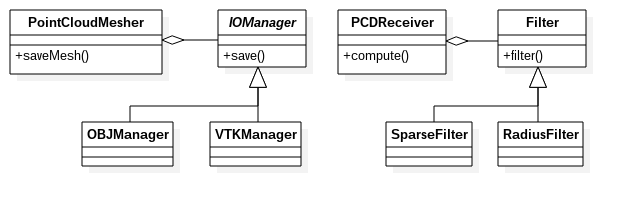
\includegraphics[width=1.05\columnwidth]{dp/strategy.png} 
    \caption{Diagramma UML del Design Pattern \texttt{Strategy}}
   \label{fig:strategy}
\end{figure}

\subsubsection{Model View Presenter}
È stato scelto il Design Pattern Model View Presenter per separare la logica dell’applicazione lato client dalla sua rappresentazione e per seguire le Android Best Practices. Il pattern è stato utilizzato nell'implementazione della "lista di mesh" dell'applicativo, come da figura \ref{fig:mvp}.
\begin{figure}[!h] 
    \centering 
    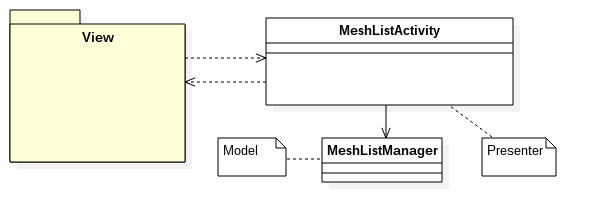
\includegraphics[width=1.0\columnwidth]{dp/mvp.png} 
    \caption{Diagramma UML del Design Pattern \texttt{MVP}}
   \label{fig:mvp}
\end{figure}
\newline
Nel sistema Android la parte \emph{View} è rappresentata da soli file XML, quindi è totalmente passiva, mentre tutta la logica viene accentrata nel \emph{Presenter}, che fa da tramite tra la  \emph{View} e il \emph{Model}.

\subsubsection{Singleton}
Il Design Pattern è stato utilizzato per controllare gli accessi alle classi che utilizzano il Logger per registrare le proprie eleborazioni. Un suo esempio d'utilizzo nell'applicativo è in figura \ref{fig:singleton}.
\begin{figure}[!h] 
    \centering 
    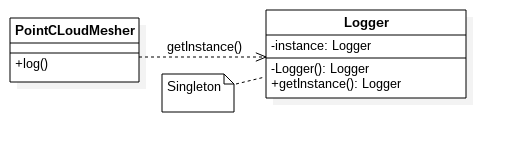
\includegraphics[width=0.9\columnwidth]{dp/singleton.png} 
    \caption{Diagramma UML del Design Pattern \texttt{Singleton}}
   \label{fig:singleton}
\end{figure}
\newline

%**************************************************************
\section{Sviluppo}

\subsection{Lato client}
\emph{VIC-Tango} è una versione rifinita e migliorata del prototipo di partenza (\emph{Samba}), del quale sono stati risolti svariati bug, immancabili allo stadio prototipale. Introduce inoltre alcune nuove funzionalità che migliorano la User experience e lasciano la porta aperta a sviluppi futuri.

\subsubsection{Firebase}
\emph{Firebase} è un \emph{framework} associato all'omonimo \emph{web service} offerto da \emph{Google} per lo scambio di messaggi tra applicazioni \emph{Android} e un \emph{server}. In particolare è stato utlizzato il servizio \emph{Firebase} di cloud messaging per la gestione e invio affidabile di messaggi a più dispositivi differenti.\\ Il suo utilizzo in VIC-Tango ha permesso di implementare un servizio di notifica da parte del server, che può così inviare messaggi asincroni al device Tango, il quale li riceverà come notifica di sistema Android, informandolo ad esempio che il Point Cloud inviato è stato elaborato e una nuova mesh è stata generata. L'utente può così continuare l'ispezione e acquisire nuovi Point Cloud e, alla ricezione della notifica, caricare e visualizzare automaticamente le mesh quando disponibili.

\subsubsection{Camera preview}
Fin dal prototipo precedente era stata introdotta una piccola preview di quanto ripreso dalla fotocamera RGB-IR. Tuttavia la funzionalità era stata implementata utilizzando una soluzione general-purpose applicabile a più dispositivi Android, che causava però problemi prestazionali e crash occasionali dell'applicativo. \\
La preview è stata quindi reimplementata utilizzando le funzionalità esposte dalle Tango API, soluzione inizialmente scartata perchè quest'ultime erano mal documentate, ottenendo un miglioramento delle prestazioni e la correzione dei bug rilevati.

\subsubsection{Visualizzazione di mesh}
Nel prototipo è stata introdotta la possibilità di caricare e visualizzare le \emph{mesh} risultato dell'elaborazione lato server di un \emph{Point Cloud}.
Una \emph{mesh} poligonale è una collezione di vertici, spigoli e facce che definiscono la forma di un oggetto poliedrico; in \emph{Samba} è ottenuta a partire dalla nuvola di punti elaborata.
Tale \emph{mesh} viene salvata dal \emph{server} in formato \emph{OBJ}, comunemente usato nelle applicazioni 3D. Dall'applicazione viene quindi richiesto di caricare e salvare nella memoria locale del tablet le mesh disponibili sul server, delle quali viene visualizzata su tablet una lista, come in figura \ref{fig:meshListView}.
\begin{figure}[!h] 
    \centering 
    \includegraphics[width=0.9\columnwidth]{varie/meshList.png} 
    \caption{La lista di \emph{mesh} visualizzata su \emph{tablet}}
   \label{fig:meshListView}
\end{figure}
\newline
Selezionando poi una singola mesh dalla lista è possibile visualizzarne il rendering tridimensionale, come in figura \ref{fig:meshViewer}. Utilizzando i comandi in alto a destra è possibile attivare/disattivare la modalità \emph{texture}, in cui al wireframe dell'oggetto vengono applicate delle textures di default, e visualizzare il volume calcolato dell'oggetto.
\begin{figure}[!h] 
    \centering 
    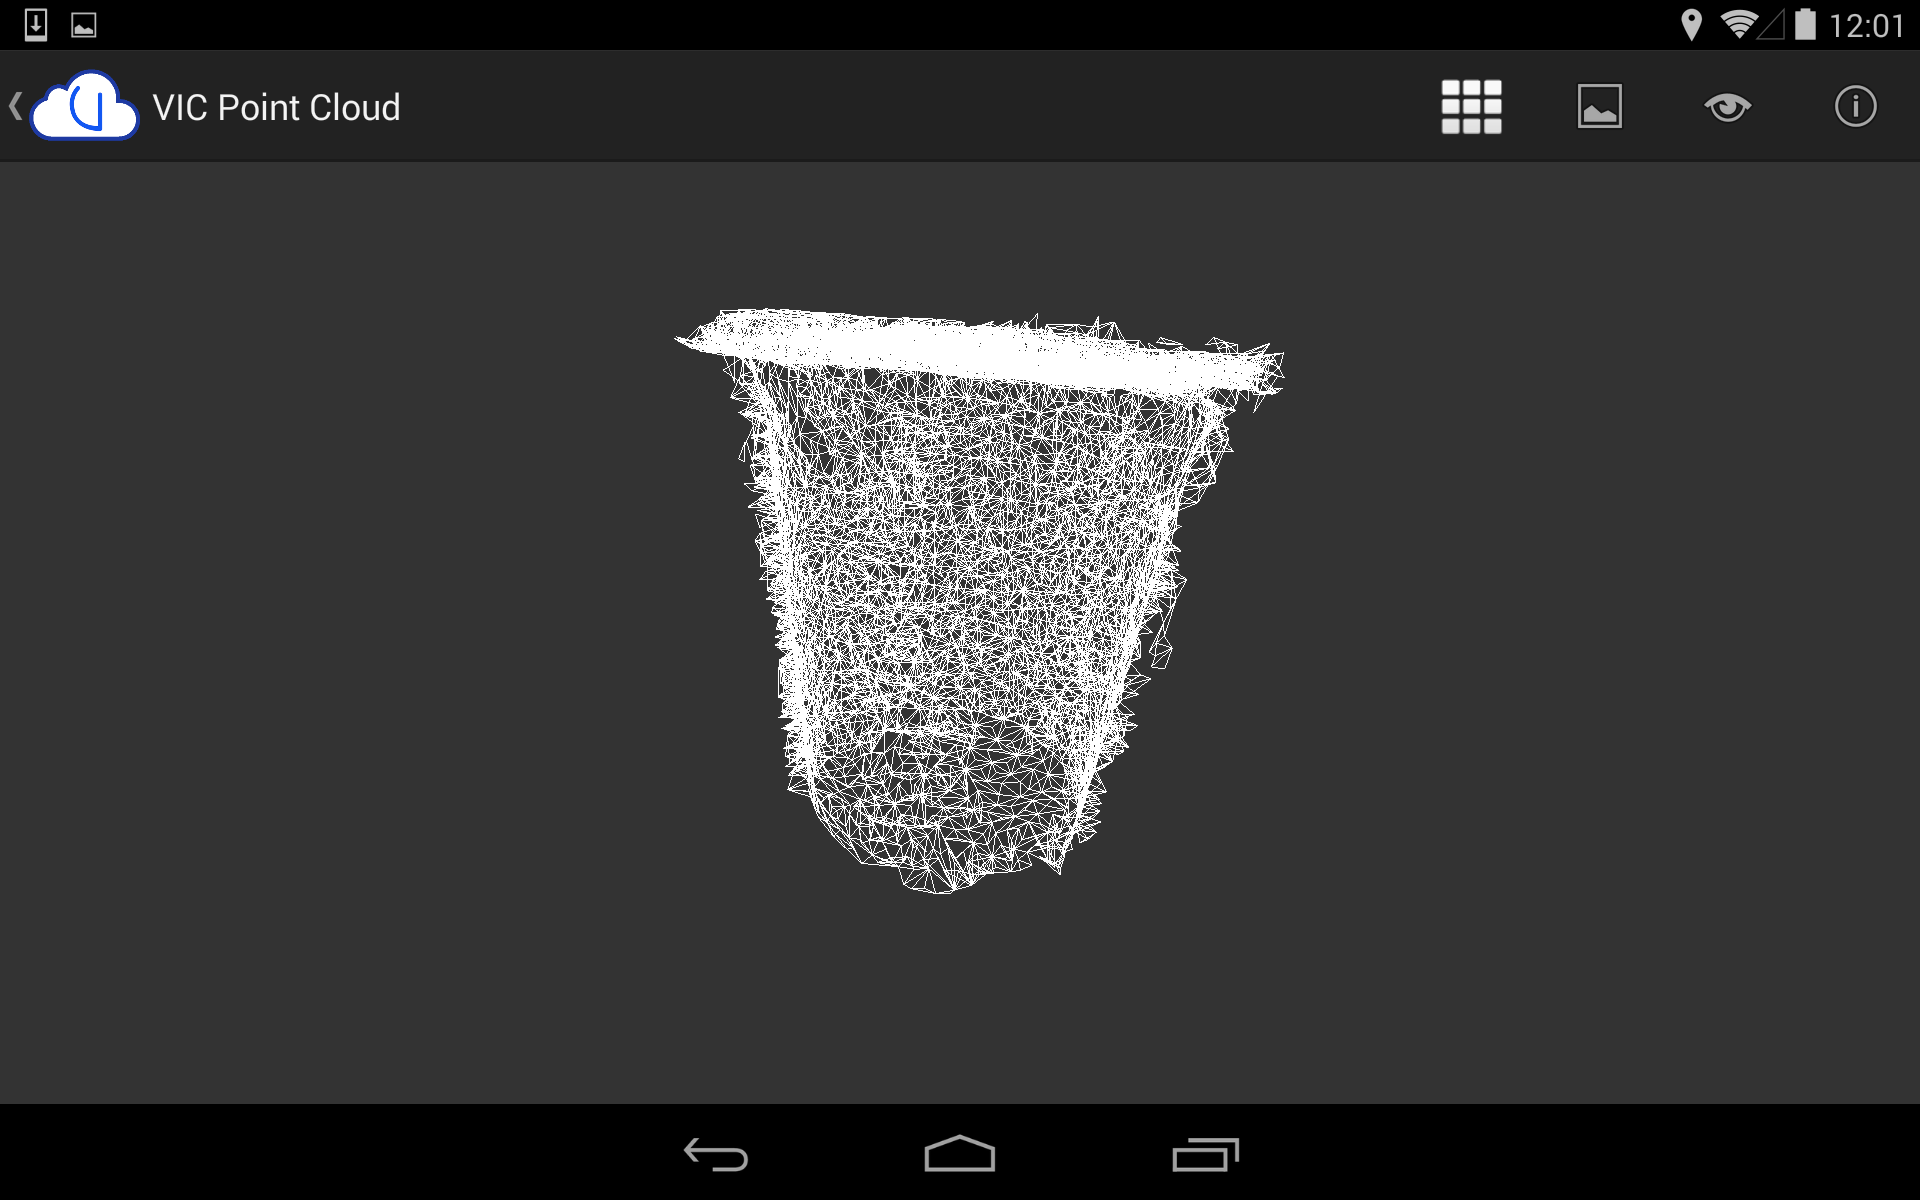
\includegraphics[width=0.9\columnwidth]{varie/meshViewer.png} 
    \caption{Rendering su \emph{tablet} di una \emph{mesh} di un cestino}
   \label{fig:meshViewer}
\end{figure}
\newline

\subsubsection{JNI e Point Cloud Registration}
\label{sec:registration}
La Java Native Interface o JNI è un framework del linguaggio Java che consente al codice Java di richiamare codice cosiddetto "nativo", ovvero specifico di un determinato sistema operativo scritto in altri linguaggi di programmazione, in particolare C/C++.\\
L'integrazione della JNI con lo sviluppo Android, in particolare il suo utilizzo nell'IDE Android Studio, è un compito tutt'altro che semplice, dato il supporto ancora scarso all'integrazione del framework con l'IDE e il build-tool Gradle.\\
Dopo svariati tentativi iniziati già i primi giorni di stage è stato infine possibile usufruire della JNI utilizzando versioni sperimentali di Android Studio e Gradle. \\
Attraverso la JNI si è provato ad importare la libreria PCL, così da poterne utilizzare le potenti funzionalità direttamente dal tablet. Purtroppo l'integrazione con il build-tool Gradle richiede un makefile apposito, compito improponibile per una libreria notevolmente complessa come PCL, le cui potenzialità sono quindi rimaste nel lato server.\\
Si è riuscito invece ad importare, date le ridotte dimensioni, una libreria per la \emph{Registration} di Point Cloud. Col termine \emph{Registration} si indica il processo che trasforma in coordinate assolute e allinea due set di Point Cloud in un unico set che minimizza le distanze tra punti corrispondenti (ad es. fig. \ref{fig:reg_example}).
\begin{figure}[!h] 
    \centering 
    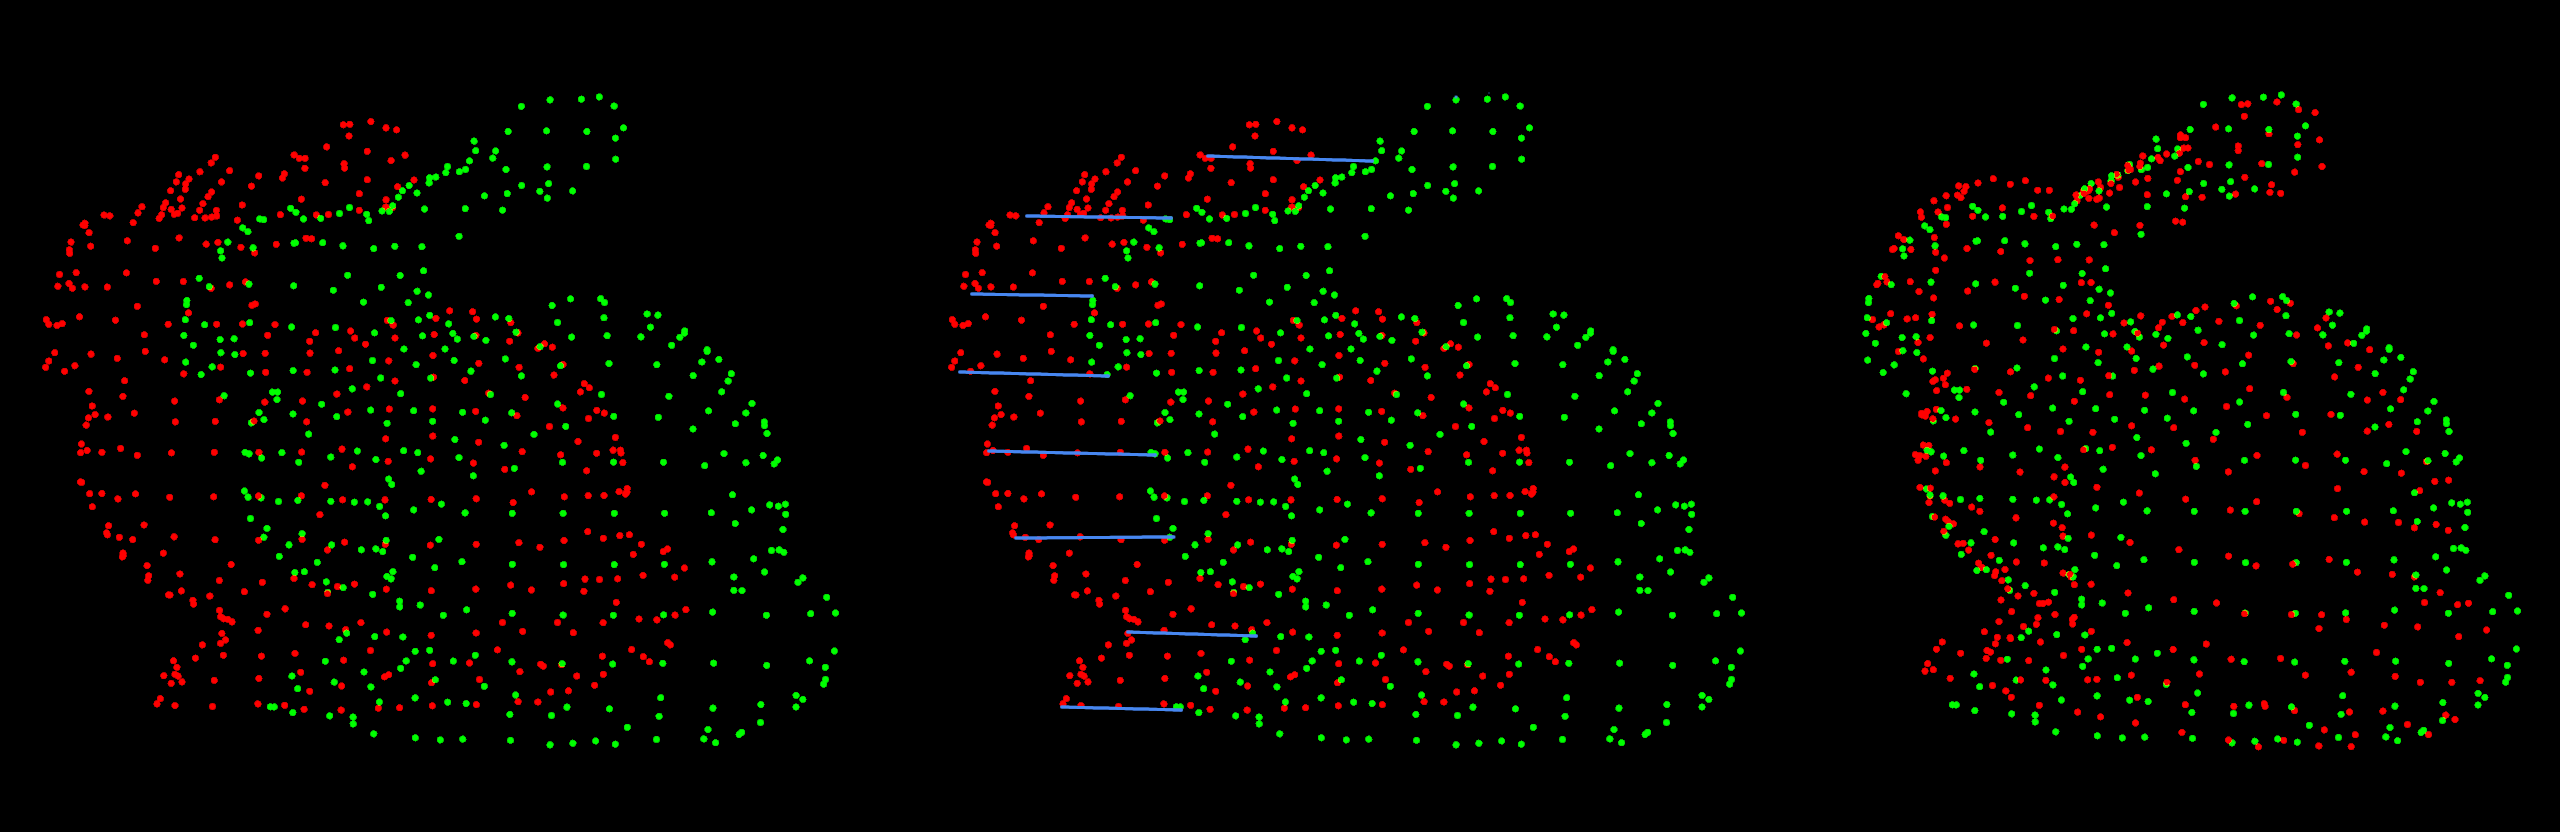
\includegraphics[width=1.0\columnwidth]{varie/registration_example.png} 
    \caption{\emph{Point Cloud Registration} tramite l'algoritmo \emph{ICP}}
    \label{fig:reg_example}
\end{figure}
\newline
La libreria in questione, GOICP, implementa una versione ottimizzata dell'algoritmo ICP (Iterative Closest Point), spesso utilizzato in applicazioni nelle quali sia necessario ricostruire una superficie tridimensionale a partire da più scansioni, che punta a minimizzare la distanza tra i punti delle due Point Cloud.\\
L'algoritmo ICP tenta di minimizzare l'errore quadratico medio (in inglese Mean Squared Error, MSE) cioè la discrepanza quadratica media fra i valori dei punti della coppia di Point Cloud, definita come:
$$
	MSE = \displaystyle\frac{\sum_{i=1}^{n} (x_i - x'_i)^2}{ n }
$$
Si è testato GOICP sulle coppie di Point Cloud acquisite con VIC-Tango, per ovviare al problemi già presentati del \emph{drifting} (fig. \ref{fig:no_drift_correction}) e del \emph{ghosting} (fig. \ref{fig:with_drift_correction}); si sono ottenuti però risultati insoddisfacenti. Sono sorti infatti i seguenti problemi:
\begin{itemize}
\item Il processo è eccessivamente dispendioso da effettuare su tablet, con tempi di elaborazione tra i 10 e i 60 secondi.
\item L'algoritmo ICP, basandosi sul MSE come valore di bontà, converge spesso lentamente e  a soluzioni errate, per colpa della grande quantità di punti planari sul pavimento, che rendono l'errore quadratico medio un valore non attendibile su cui basare il successo di una \emph{Registration} 
\end{itemize}
Come si vede in figura \ref{fig:goicp} l'algoritmo, pur ottenendo un basso valore di MSE, non effettua la \emph{Registration} desiderata, dato che vengono allineati perlopiù i punti planari.
\begin{figure}[htp] 
    \centering
    \subfloat[Prima scansione]{%
        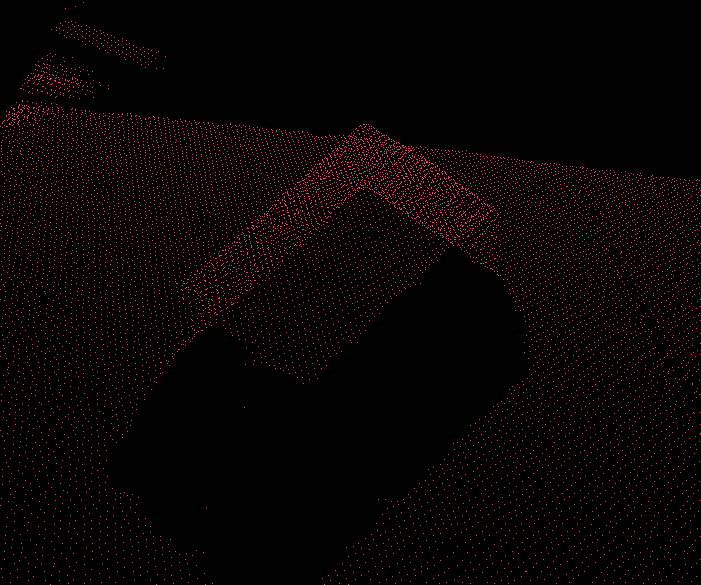
\includegraphics[width=0.5\columnwidth]{varie/to_align_left.png} 
    	\label{fig:goicp_left}
    }%
    \hfill%
    \subfloat[Seconda scansione]{%
        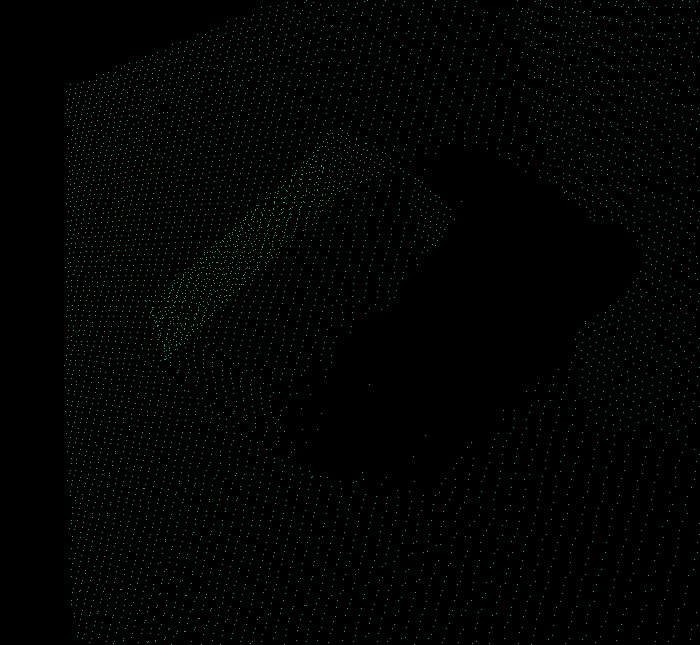
\includegraphics[height=0.42\columnwidth]{varie/to_align_right.png} 
    	\label{fig:goicp_right}
    }%
    \hfill%
    \subfloat[Risultato di GOIPC]{%
        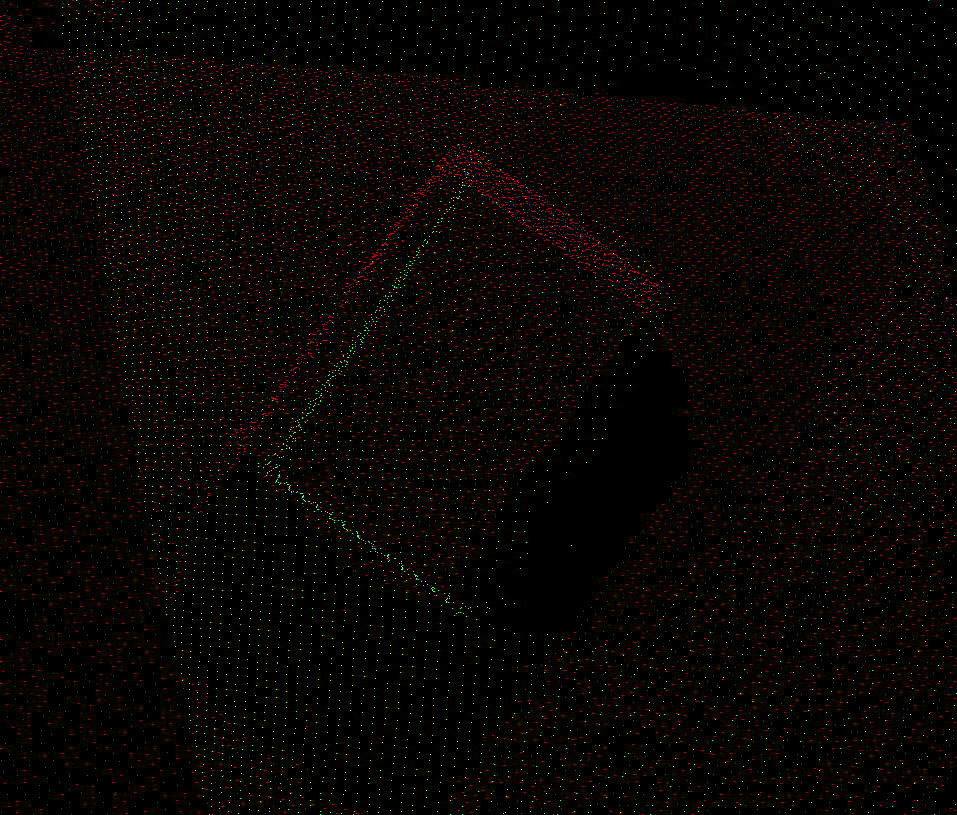
\includegraphics[width=0.6\columnwidth]{varie/goicp.png} 
    	\label{fig:goicp}
    }%
    \caption{Errore nella \emph{Registration} con \emph{GOICP}}
\end{figure}
\newline

\noindent
Per questi motivi la \emph{registration} tramite GOICP è rimasta in uno stadio prototipale, che necessita di almeno una delle seguenti correzioni:
\begin{itemize}
\item Trovare una misura più adatta del MSE per valutare la convergenza dell'algoritmo ICP
\item Alternativamente, eliminare dal Point Cloud i punti planari appartenenti al pavimento così da poter utilizzare l'errore quadratico medio come affidabile valore di convergenza
\item Ottimizzare GOICP o implementare un algoritmo ICP ad hoc per ridurre drasticamente i tempi di elaborazione
\end{itemize}
\noindent
Tali correzioni trattano problemi non triviali, che l'esiguo tempo di tirocinio rimasto non mi ha permesso di affrontare adeguatamente. La Point Cloud Registration rimane quindi una funzionalità necessaria ad assicurare un'affidabile e corretta ricostruzione degli oggetti scansionati, aperta a sviluppi futuri.

\subsection{Lato server}
Il lato server dell'applicazione si occupa di ricevere dai \emph{Tango device} i Point Cloud acquisiti, elaborarli utilizzando la libreria PCL per estrarre i punti rappresentanti il solo oggetto scansionato, produrre una mesh dell'oggetto così ottenuto e calcolarne il volume. Invia poi quando necessario i risultati elaborati ai dispositivi che li richiedono.\\
Quando un Point Cloud viene ricevuto dal server tramite una richiesta HTTP POST, inserito in un oggetto JSON, viene salvato in un file PCD. Il formato PCD (Point Cloud Data) usato nella libreria PCL è molto semplice: è formato da un header contenente alcune informazioni utili come il numero totale di punti e il tipo e numero di valori associati ad ogni punto; segue poi l'effettivo Point Cloud codificato riga per riga, dove ogni riga contiene una successione di valori che rappresenta un punto.\\
Il file salvato viene poi elaborato sfruttando la libreria PCL.

\subsection{Elaborazione di un Point Cloud}

La nuvola di punti salvata in un file PCD viene elaborata da un applicativo scritto in C++ che sfrutta le numerose funzionalità della PCL.
L'elaborazione di un Point Cloud è composta di più passi sequenziali:
\begin{enumerate}
\item Viene caricato il nuovo Point Cloud da file PCD salvato localmente
\item Vengono rimossi i punti isolati della nuvola attraverso la libreria Sparse Filtering
\item Vengono rimossi i punti troppo esterni della nuvola attraverso la libreria Radius Filtering 
\item Vengono rimossi i punti che corrispondono al piano del pavimento attraverso la libreria Ground Filtering
\item Viene effettuato il \emph{downsample} del \emph{dataset} attraverso la libreria Voxel Filtering
\item Viene estratto il cluster maggiore dai punti rimanenti attraverso la libreria Cluster Extraction
\item Viene effettuato il meshing del cluster estratto, e la mesh viene salvata in due file OBJ (per la visualizzazione lato client) e VTK (per il calcolo del volume)
\item Viene calcolato e salvato il volume della mesh prodotta
\end{enumerate}
Per ogni passo di filtraggio la nuvola di punti viene salvata su un distinto file PCD, per poter analizzare visivamente la bontà dell'elaborazione.
Di seguito vengono descritti in dettaglio filtri applicati e il processo di meshing.

\subsubsection{Sparse filtering}
Questo primo passo di filtraggio si occupa di rimuovere dal Point Cloud i punti isolati. Per ogni punto viene effettuata una analisi statistica della distanza media dai suoi vicini. I punti la cui distanza dai vicini supera un certo valore sono quindi isolati e possono essere eliminati dalla nuvola.
Un esempio di tale tecnica, sul quale si basa l'implementazione di questo filtro, è lo "Statistical Outlier Removal\footcite{http://pointclouds.org/documentation/tutorials/statistical_outlier.php/statistical-outlier-removal}" di PCL.\\
In figura \ref{fig:sparse} vediamo i risultati di tale filtro, con una rimozione di circa 10.000 punti.
\begin{figure}[!h] 
    \centering 
    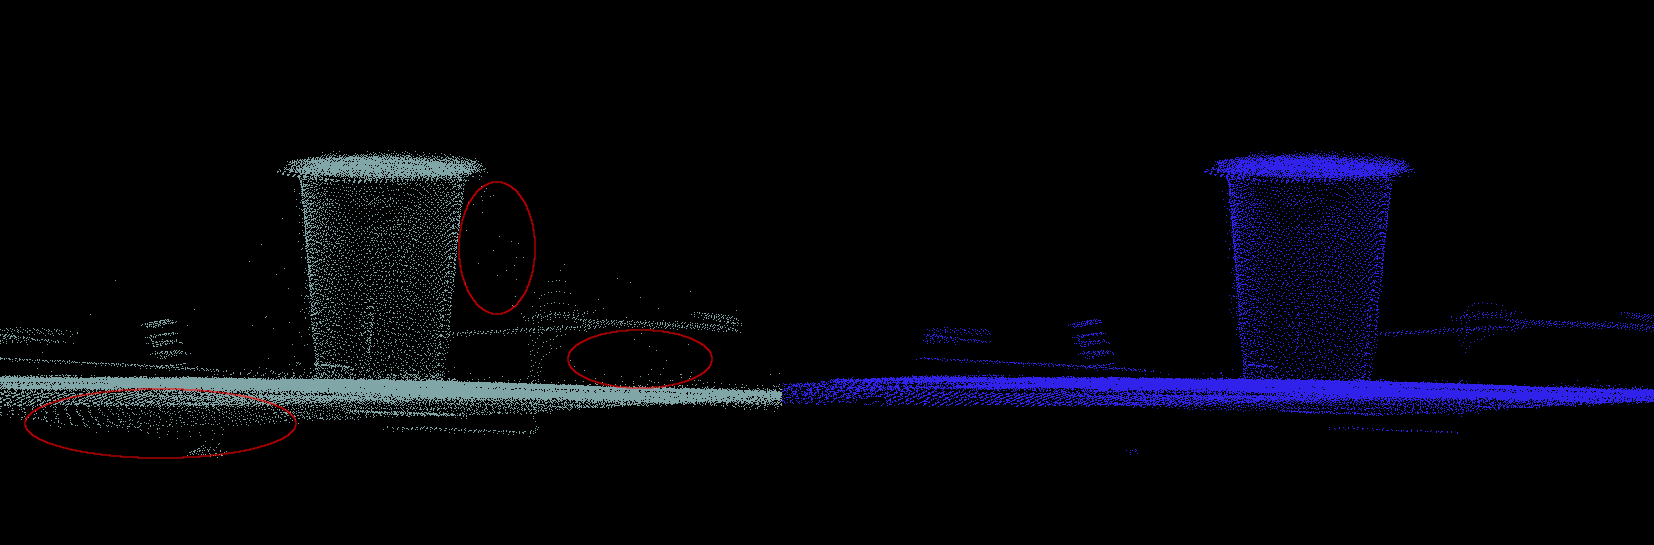
\includegraphics[width=1.0\columnwidth]{varie/sparse.png} 
    \caption{\emph{Sparse filtering}}
    \label{fig:sparse}
\end{figure}
\subsubsection{Radius filtering}
Questo passo di filtraggio si occupa di eliminare i punti troppo distanti dal centro, che solitamente appartengono alle pareti circostanti o comunque ad oggetti diversi da quello scansionato, che sarà sempre verso il centro della nuvola.\\
Partendo da questo presupposto, il filtro calcola il punto centrale del Point Cloud, media del valore di tutti i punti, e procede con l'eliminare i punti che superano una certa distanza (\emph{radius}), attraverso l'algoritmo PCL "PassThrough Filter\footcite{http://pointclouds.org/documentation/tutorials/passthrough.php/passthrough}", fino a che non è stata eliminata una definita percentuale del point set iniziale.\\
In figura \ref{fig:radius} vediamo i risultati di tale filtro, con una rimozione di circa 24.000 punti.
\begin{figure}[!h] 
    \centering 
    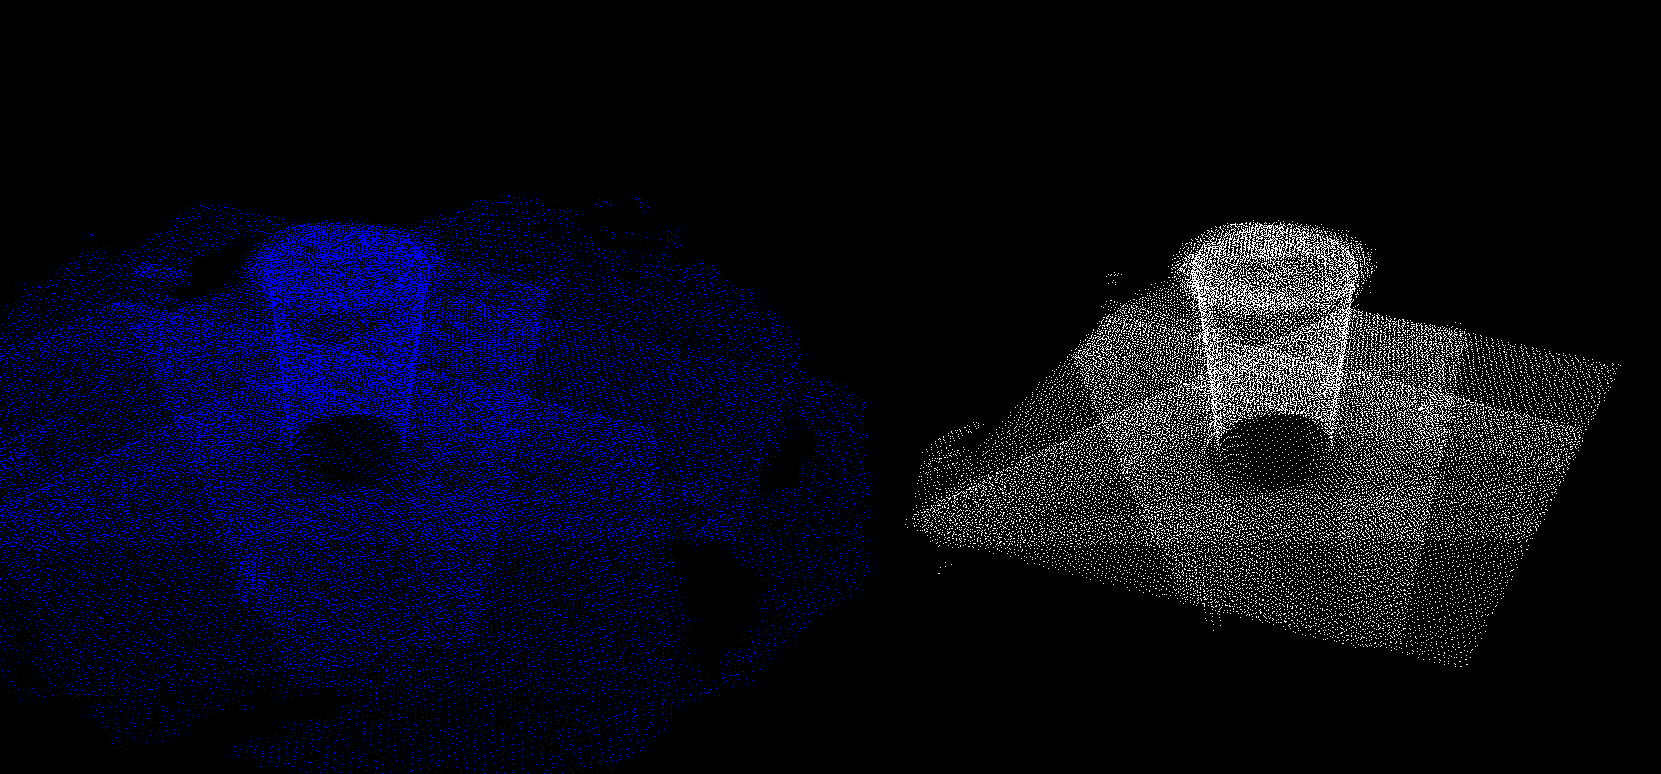
\includegraphics[width=1.0\columnwidth]{varie/radius.png} 
    \caption{\emph{Radius filtering}}
    \label{fig:radius}
\end{figure}
\subsubsection{Ground filtering}
Questo passo di filtraggio si occupa di eliminare i punti planari appartenenti al pavimento, problema che si è rilevato essere uno dei più difficili da trattare. 
In primo luogo non sempre c'è un unico componente planare che rappresenta il pavimento, ma solitamente ve n'è più d'uno, a causa delle imprecisioni nell'acquisizione dei Point Cloud lato client. Per l'implementazione del filtro si è fatto uso degli algoritmi di \emph{segmentation} di PCL (ad es. "Planar segmentation\footcite{http://pointclouds.org/documentation/tutorials/planar_segmentation.php}"), che consentono di estrarre i punti della nuvola che giacciono sullo stesso piano. Senza ulteriori aggiustamenti però l'algoritmo elimina anche piani utili, come il lato superiore di una scatola o di un tavolo.
Si è reso quindi necessario applicare i seguenti passi:
\begin{enumerate}
\item Calcolare l'altezza del Point Cloud e dividere la parte superiore da quella inferiore, che deve contenere il pavimento
\item Applicare l'algoritmo di \emph{planar segmentation} alla sotto-nuvola estratta fino a che non è stato eliminato un numero adeguato di punti
\item Ricongiungere la parte inferiore filtrata alla parte superiore del Point Cloud
\end{enumerate}
Il filtro così impostato ottiene ottimi risultati nella maggior parte dei casi. Tuttavia se il Point Cloud originale presenta troppo  \emph{drifting}, e i piani del pavimento sono molto distanti tra loro, diventa impossibile eliminarli senza togliere anche punti importanti dell'oggetto scansionato.\\
In figura \ref{fig:ground} vediamo i risultati di tale filtro, applicato ad un Point Cloud già sottoposto ai filtri precedenti, con una rimozione di circa 50.000 punti.
\begin{figure}[!h] 
    \centering 
    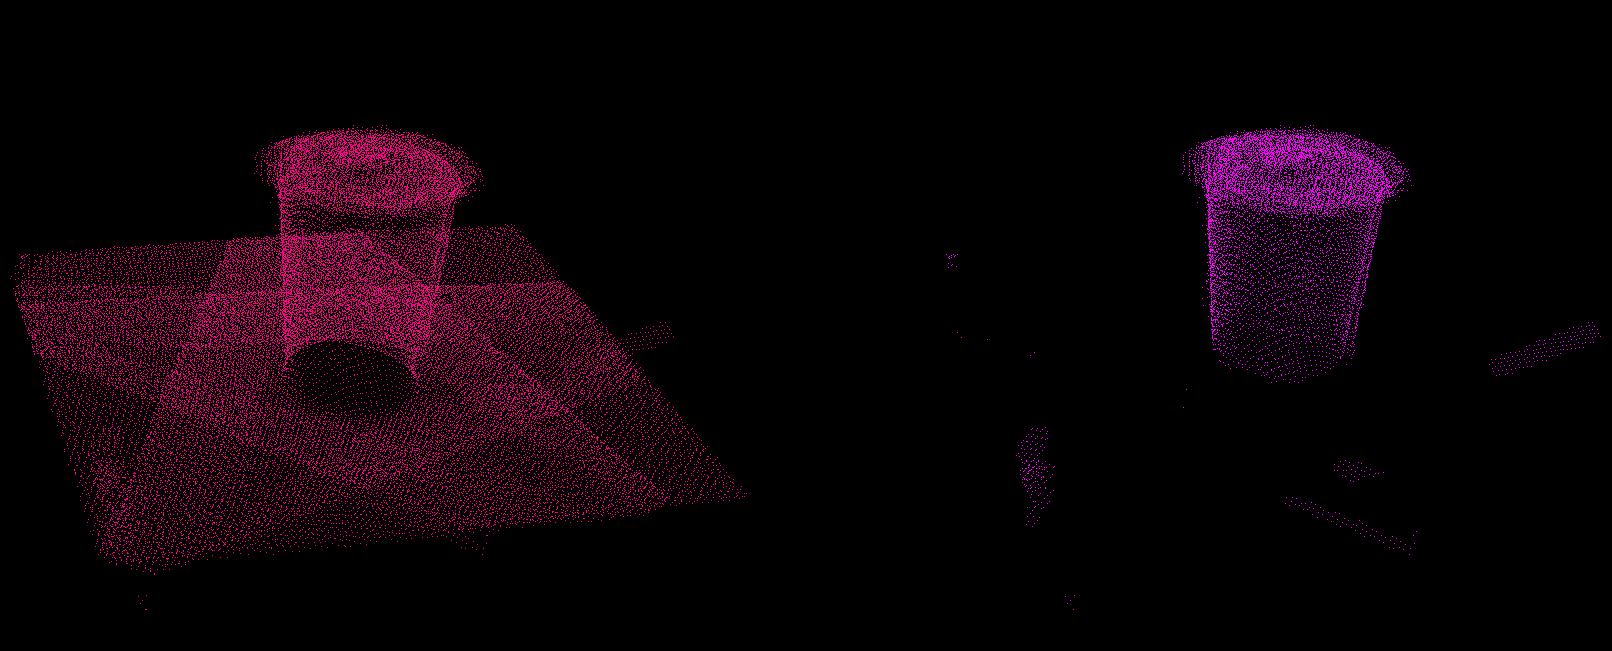
\includegraphics[width=1.0\columnwidth]{varie/ground.png} 
    \caption{\emph{Ground filtering}}
    \label{fig:ground}
\end{figure}

\subsubsection{Voxel filtering}
Questo passo di filtraggio si occupa di eliminare i punti doppi e ridurre le dimensioni del Point Cloud per il futuro meshing. Il filtro utilizza la stessa tecnica già implementata nel lato client, cioè suddividere lo spazio in tanti \emph{voxel} cubici e  calcolare il punto medio di ogni voxel come approssimazione dei punti che ricadono al suo interno. L'implemetazione prende spunto dall'esempio di PCL "VoxelGrid Filter\footcite{http://pointclouds.org/documentation/tutorials/voxel_grid.php}".
Per i risultati del \emph{voxel filtering} si rimanda alle figure \ref{fig:low_voxeling} e \ref{fig:high_voxeling}.
\subsubsection{Cluster extraction}
L'ultimo passaggio prima del meshing è il \emph{Cluster extraction}, cioè il completo isolamento della nuvola di punti rappresentante oggetto in ispezione.
L'algoritmo PCL "\emph{Euclidean Cluster Extraction\footcite{http://www.pointclouds.org/documentation/tutorials/cluster_extraction.php}}" su cui si base quest'ultimo step di filtraggio suddivide lo spazio del Point Cloud in più parti ed analizzandone statisticamente la densità per ogni parte, riesce a determinare quali sono  gli aggregati di punti nella nuvola, distinguibili gli uni dagli altri.
L'algoritmo suddivide quindi la nuvola in più cluster, e ne estrae quello di maggiori dimensioni. Questo filtraggio finale indispensabile al passo successivo di meshing, perchè elimina dal Point Cloud tutti gli elementi estranei all'oggetto.\\
In figura \ref{fig:cluster} vediamo i risultati di tale filtro, applicato ad un Point Cloud già sottoposto ai filtri precedenti, con una rimozione di circa 4.000 punti. Sono evidenziati in figura alcuni piccoli gruppi di punti che è necessario eliminare, che rappresentano degli artefatti inesistenti nel mondo reale, ma che sono immancabilmente presenti nelle scansioni di un oggetto. L'origine di tali anomalie non è ancora chiara, probabilmente sono causate da riflessi del pavimento.
\begin{figure}[!h] 
    \centering 
    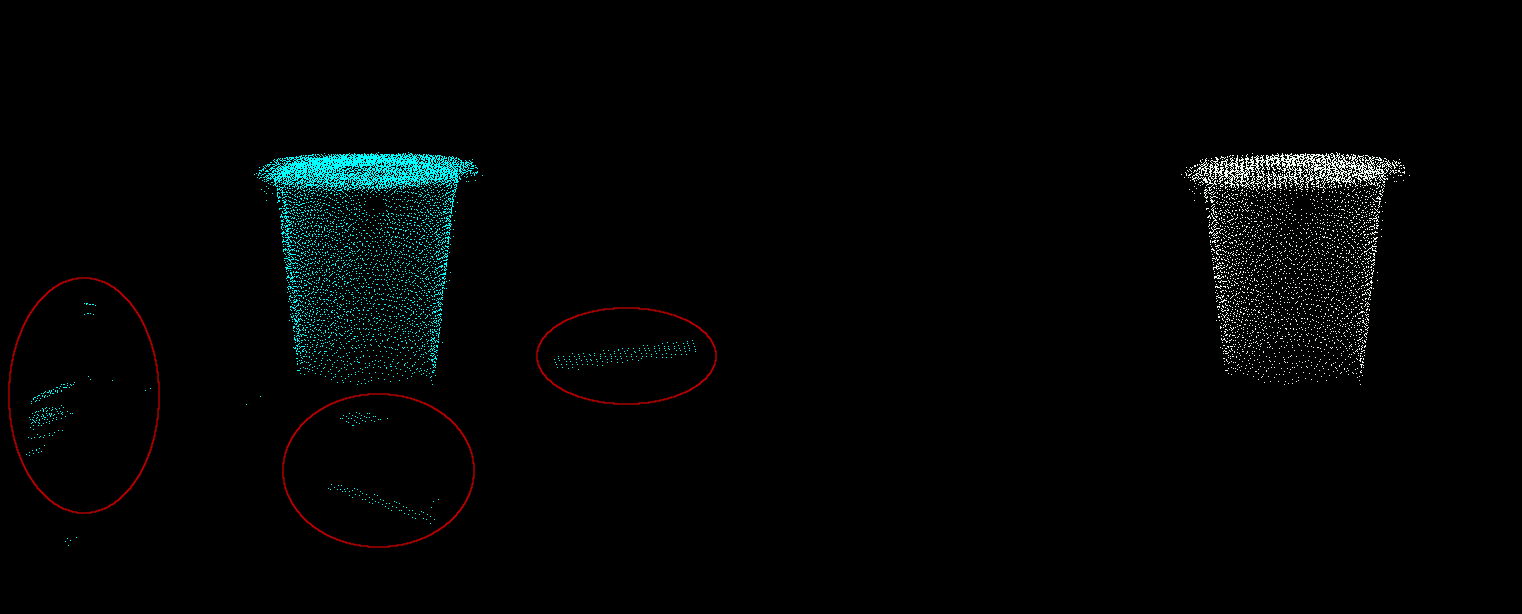
\includegraphics[width=1.0\columnwidth]{varie/cluster.png} 
    \caption{\emph{Cluster extraction}}
    \label{fig:cluster}
\end{figure}

\subsubsection{Meshing}
Una volta ottenuti i punti della nuvola rappresentanti il solo oggetto scansionato, si può procedere col generarne una mesh tridimensionale.
Il processo sfrutta un algoritmo greedy di PCL, la "\emph{Greedy Projection Triangulation\footcite{http://www.pointclouds.org/documentation/tutorials/greedy_projection.php}}", che, connettendo ogni punto ai propri vicini, genera un mesh composta da migliaia di triangoli che approssima la superficie reale dell'oggetto.
In figura \ref{fig:mesh} vediamo i risultati del processo di meshing applicato ad un Point Cloud già sottoposto ai filtri precedenti.
\begin{figure}[!h] 
    \centering 
    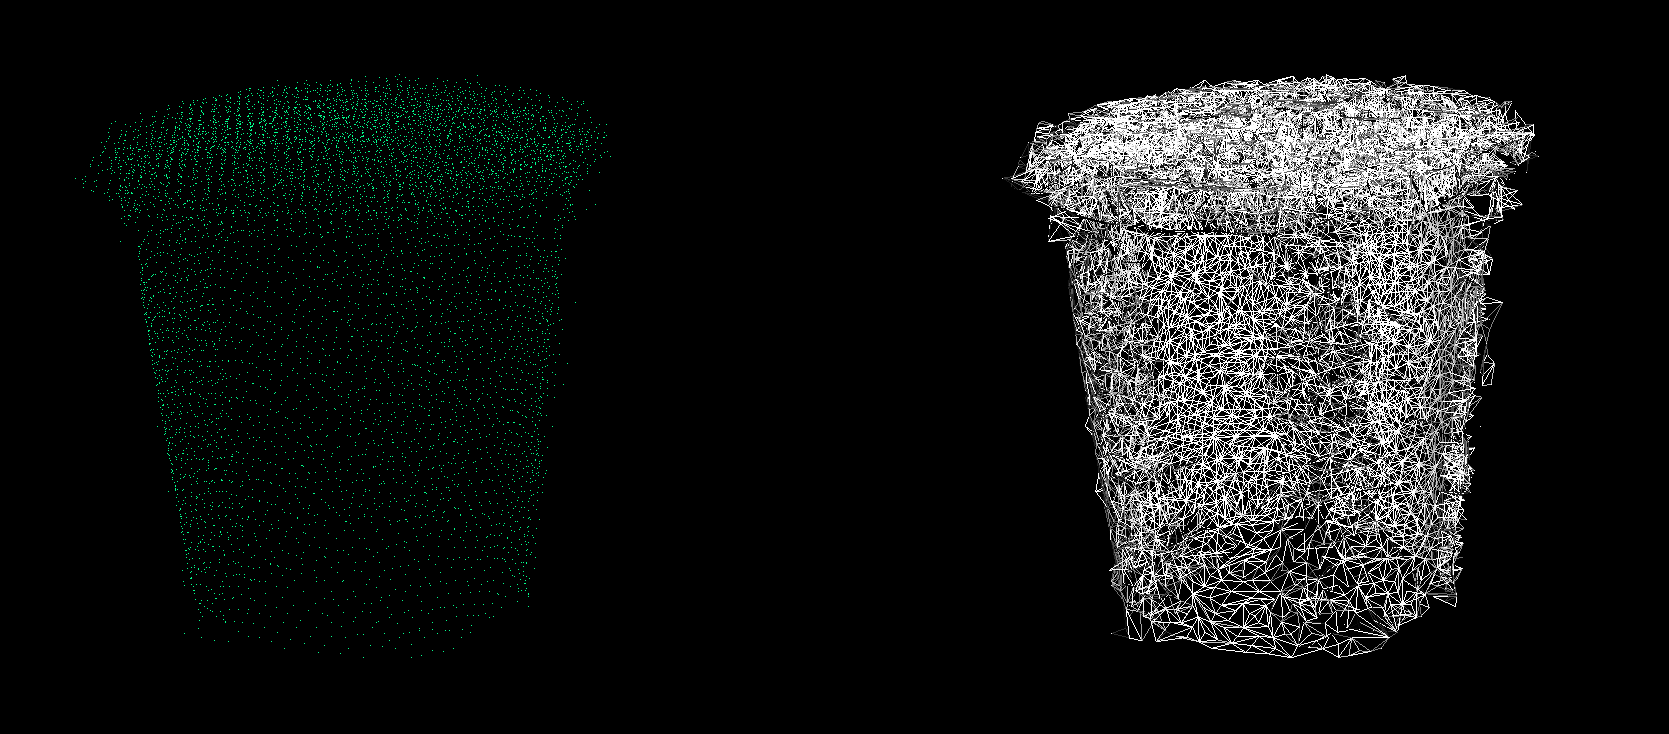
\includegraphics[width=1.0\columnwidth]{varie/mesh.png} 
    \caption{\emph{Meshing} di un \emph{Point Cloud}}
    \label{fig:mesh}
\end{figure}
\newline
La mesh così ottenuta non è una superficie chiusa, spesso infatti le scansioni non riescono a catturare tutti i punti di un oggetto, e manca completamente il piano di base dell'oggetto scansionato, che non è possibile rilevare. Ciò non influisce particolarmente sul successivo calcolo del volume.

\subsection{Calcolo del volume}
Una volta generata la mesh è possibile calcolarne il volume sfruttando il risultato pubblicato da Cha Zhang e Tsuhan Chen nel loro paper\footcite{http://research.microsoft.com/en-us/um/people/chazhang/publications/icip01_ChaZhang.pdf}. Viene calcolato, per ogni triangolo che compone la \emph{mesh}, il volume con segno del tetraedro che ha il triangolo stesso come base e il quarto vertice in un punto fissato, scelto internamente alla \emph{mesh}, per evitare eventuali problemi di instabilità numerica. Il segno del volume è dato dalla direzione della normale al piano del triangolo. Questi volumi, sommati tra loro, restituiscono il volume convesso della \emph{mesh}.\\
Il calcolo del volume, nella sua semplicità e velocità d'elaborazione, pone però delle condizioni sulla qualità della mesh:
\begin{itemize}
\item La superficie non necessita di essere chiusa, ma il calcolo ne beneficierebbe
\item Il punto scelto come quarto vertice del tetraedro deve appartenere alla mesh
\item La mesh non deve contenere triangoli che si sovrappongono o si intersecano
\end{itemize}
La bontà del calcolo dipende quindi molto dalla qualità del Point Cloud prima del meshing, che dev'essere quanto più assente da fenomeni di \emph{ghosting}, \emph{drifting} e in generale da artefatti e punti sparsi che non riflettono la vera forma dell'oggetto ispezionato.
